\section{Horizontes Lejanos}
\subsection{Introducci\'on}

En este problema en particular hay que diseñar un software de arquitectura sobre el m\'odulo de Edificios 2D. En este, se representan a los edificios como un conjunto de rect\'angulos apoyados sobre un mismo eje. \\
Ahora bien, el problema consiste en dibujar el perfil del conjunto de edificios (es decir el contorno que se ver\'ia desde el horizonte) eliminando las l\'ineas ocultas. 
\\
\\
El siguiente es un ejemplo del problema con su respectiva soluci\'on: \\ \\

\begin{tabular}{| l |}
\hline
Entada \\ \hline
4 \\ 
9 11 15 \\ 
7 12 10 \\ 
2 5 5 \\ 
10 10 14 \\ \hline
\end{tabular}


\begin{figure}[H]
  \centering
	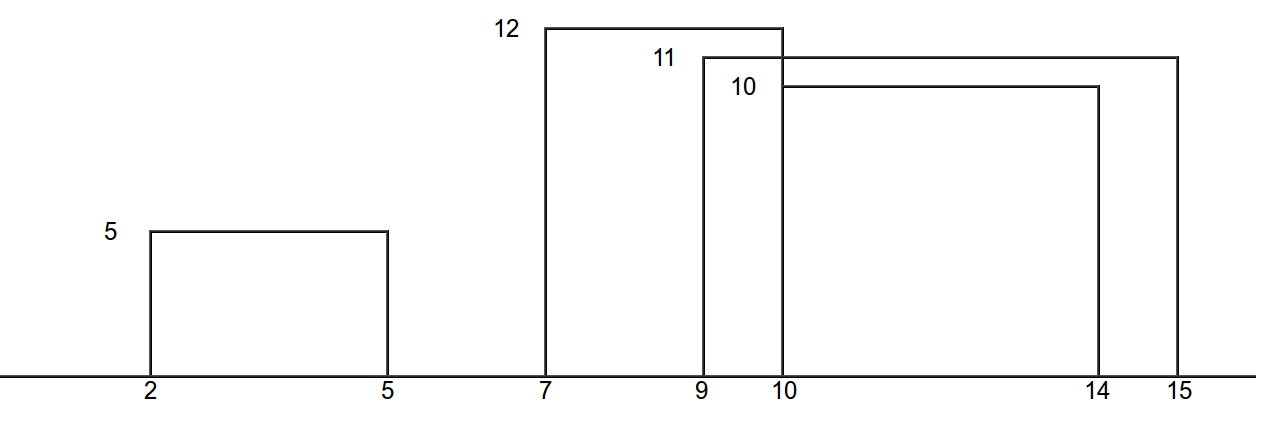
\includegraphics[scale=0.27]{./Imagenes/Ej2/Ejemplo-Entrada.png} 
\end{figure}



Al eliminar las lineas internas, la vista desde el ''horizonte'' ser\'a la siguiente: \\ \\


\begin{figure}[H]
  \centering
	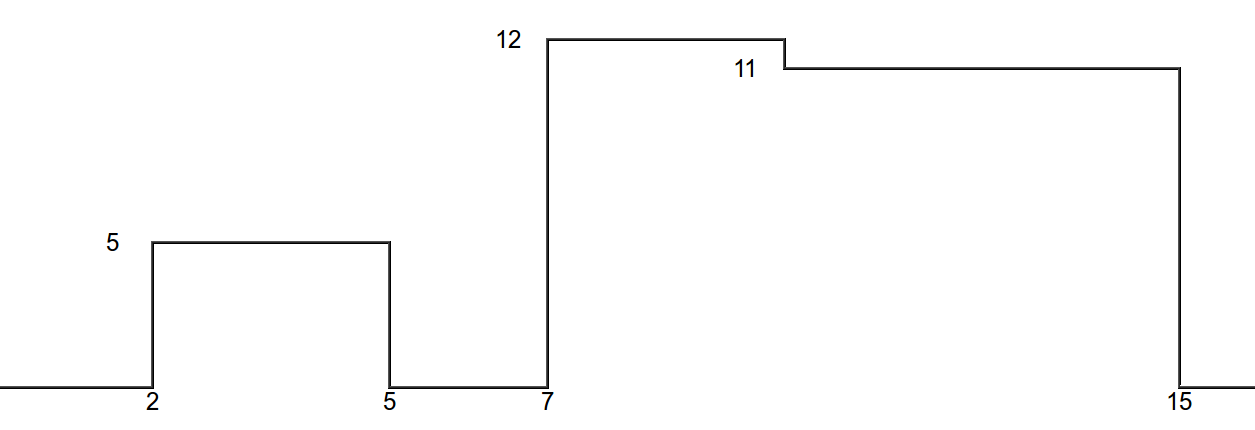
\includegraphics[scale=0.27]{./Imagenes/Ej2/Ejemplo-Salida.png} 
\end{figure}


La salida del algoritmo solo deber\'a contener una l\'inea con una sucesi\'on de pares de valores (x, y) representando cada cambio de altura en el horizonte, donde \textbf{x} representa la coordenada horizontal en donde se produce el cambio de altura e \textbf{y} representa la nueva altura a partir de \textbf{x}. Adicionalmente, nos piden que dichos pares est\'en ordenados de menor a mayor por su coordenada \textbf{x}.
\\
\\
Luego, la salida para el ejemplo anterior sera la siguiente:
\quad 
\begin{tabular}{| l |}
\hline
(2 5), (5 0), (7 12), (10 11), (15 0) \\ \hline
\end{tabular}



\subsection{Desarrollo}

Decidimos dividir el problema en dos partes: 
\begin{itemize}
\item Identificar los ''flancos ascendentes'' $\rightarrow$ los cambios de altura hacia una altura mayor.
\item Identificar los ''flancos descendentes'' $\rightarrow$ los cambios de altura hacia una altura menor.
\end{itemize}
En el ejemplo anterior: \quad \quad
\begin{tabular}{| l | l |}
\hline
Ascendentes:   & (2 5), (7 12) \\ \hline
Descendentes:  & (5 0), (10 11), (15, 0) \\ \hline
\end{tabular}
\\
\\
Luego combinaremos los dos para devolver la salida final.
\\
\\
Como en realidad, ambas partes son similares, ya que un cambio de altura en la posici\'on \textbf{x} hacia una altura menor mirando el gr\'afico de izquierda a derecha, ser\'a un cambio de altura hacia una altura mayor mirando el gr\'afico de derecha a izquierda (en la misma posici\'on x). \\
Luego las unicas diferencias entre ambas ser\'a el criterio de orden para el vector y la manera de chequear si dos efificios se superponen o no.


\begin{codebox}
\Procname{\textbf{Pseudocodigo:}}
\li Ordenamos el vector de edificios.
\li Creamos un heap ordenado por mayor altura (vacio).
\li Agregamos al heap el \textbf{piso} (edificio de altura 0 que abarca desde la posicion 0 hasta el final)
\li Para cada edificio \textbf{a} del vector ya ordenado
\li \ \ \ \ (*) Tomamos el mayor elemento del heap (llamese \textbf{b}).
\li \ \ \ \ Si \textbf{a} y \textbf{b} no se superponen, sacamos a \textbf{b} del heap y volvemos a (*)
\li \ \ \ \ Si \textbf{a} es más alto que \textbf{b}, anotaremos un flanco ascendente donde comienza \textbf{a}
\li \ \ \ \ Agregamos \textbf{a} al heap.
\end{codebox}

\begin{codebox}
\Procname{\textbf{Orden en FlancosAscendentes:}}
\li El que tenga menor izquierda primero 
\li El que tenga mayor altura primero
\li El que tenga menor derecha primero
\end{codebox}
En el ejemplo anterior, los edificios quedar\'an en el siguiente orden:
\begin{tabular}{| l |}
\hline
(2 5 5), (7 12 10), (9 11 15), (10 10 14)\\  \hline
\end{tabular}


\begin{codebox}
\Procname{\textbf{Orden en FlancosDescendentes:}}
\li El que tenga mayor derecha primero
\li El que tenga mayor altura primero
\li El que tenga mayor izquierda primero
\end{codebox}
En el ejemplo anterior, los edificios quedar\'an en el siguiente orden:
\begin{tabular}{| l |}
\hline
(9 11 15), (10 10 14), (7 12 10), (2 5 5)   \\  \hline
\end{tabular}

\begin{codebox}
\Procname{\textbf{Superposicion}}
\textbf{A} se superpone con \textbf{B} si la parte izquierda de \textbf{A} es menor que la parte derecha de \textbf{B}
\end{codebox}



\begin{figure}[H]
\centering
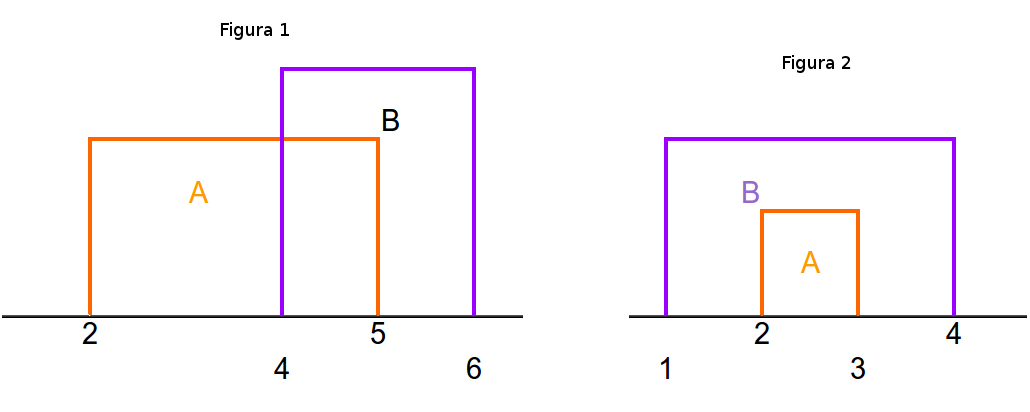
\includegraphics[scale=0.36]{./Imagenes/Ej2/ab3.png} 
%\caption{B se superpone con A}
\end{figure}

\begin{figure}[H]
\centering
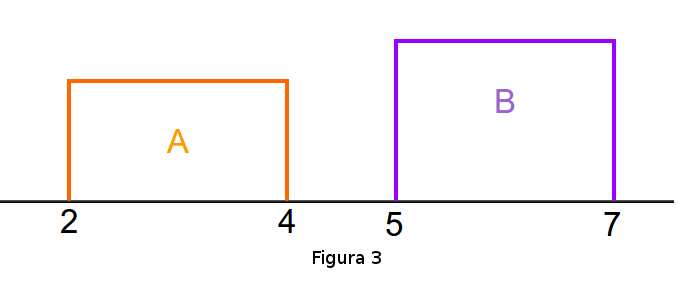
\includegraphics[scale=0.36]{./Imagenes/Ej2/ab4.png} 
%\caption{B se superpone con A}
\end{figure}

\subsection{Demostraci\'on de correctitud} 

Antes que nada veamos que no puede existir un cambio de altura en el horizonte en una posici\'on que no sea el inicio o el final de un edificio. Debido a que los edificios son rectangulares y con alturas $>$ 0, las únicas posiciones donde pueden cambiar de altura son en su lado izquierdo o derecho.
\\
\\
Analizemos entonces cuando es que hay un cambio de altura hacia una altura mayor:
\\
En primera instancia podr\'iamos decir que cada vez que empieza un edificio \textbf{A} (el valor $izq$ del mismo) hay un flanco ascendente, pero esta afirmaci\'on no es verdadera cuando A se ''superpone'' con otro edificio \textbf{B} m\'as alto que A, ya que en el horizonte, B estar\'ia tapando la primera parte de A. 
\\
\\
Luego, analizemos nuestro algoritmo para ver que se cumple la siguiente condici\'on:
\\
Cambio de altura en A.izq $ \Leftrightarrow \not \exists B \in $edificios tal que $B.alt > A.alt$
\\
\\
Como podemos ver en el pseudoc\'odigo, la idea general de resoluci\'on es ir tomando los edificios de a uno (de manera ordenada) y comparar el mismo con los que ya hallamos iterado.
\\
\\
Lo primero que hacemos es agregar ''el piso'' al heap, con esto nos aseguramos de tener siempre un elemento en el heap, ya que al abarcar desde el inicio hasta el final se estar\'ia ''superponiendo'' con todos los edificios y por lo tanto nunca entrar\'a al \textbf{if} que chequea si no se superponen (y por consiguiente nunca ser\'a sacado del heap). Con esto nos estamos asegurando la terminaci\'on del \textbf{while}.
\\
\\
Lo que hacemos entonces es ordenar los edificios de menor a mayor segun su valor de inicio ($izq$). De esta manera podremos iterarlos de manera ordenada.
\\
\\ 
Sean $a_1$ $a_2$ $a_3$ .. $a_n$ todos los edificios ya ordenados.
\\
\\
Al iterar $a_1$, estamos comparando si se superpone con el piso (ya que es el \'unico elemento del heap), esto siempre es cierto , y como la altura del piso es 0, siempre habr\'a un flanco ascendente al comienzo del primer edificio (**).
\\
\\

Al iterar $a_i$, lo que hacemos es chequear si es mas alto que todos los edificios que estan dentro del heap con los que se superpone. En particular
%(para bajar la complejidad ESTO TAMBIEN LO EXPLICARIA MEJOR)
en la primera posici\'on del heap siempre estar\'a el edificio m\'as alto, llamese \textbf{B}, y tendremos 2 casos
\begin{itemize}
\item Si $a_i$ se superpone con B, pasamos a chequear la altura
\begin{itemize}
\item Si no se superponen, debemos seguir buscando en el heap un edificio con uno con el que si lo haga. Siempre existir\'a uno, el piso, que ser\'a el \'ultimo por tener altura 0. 
\\
Adicionalmente como B no se superpone con a$_i$ (B.der $<$ a$_i$.izq), ning\'un a$_k$ con k $>$ i lo har\'a tampoco, porque a$_i$.izq $\leq$ a$_k$.izq con k $>$ i (por el orden que le dimos). Seremos libres entonces de quitar a B del heap para evitar futuras comparaciones en vano.
\end{itemize}
\item Si a$_i$ es m\'as alto que B, habr\'a un flanco ascendente, ya que dentro del heap todos los edificios ser\'an mas bajos que B.
\item Si B es m\'as alto que a$_i$, no tendremos cambio de altura al comienzo del edificio a$_i$ ya que el mismo estar\'a ''tapado'' por B.
\end{itemize}

Como nuestro algoritmo recorre el inicio de todos los edificios, chequea que no exista un edificio m\'as alto con el que se superponga y solo entonces agenda un cambio de altura.
Y no puede existir un cambio de altura hacia una altura m\'as alta en otra posicion que no sea al comienzo de un edificio, podemos decir que nuestro algoritmo registra todos los flancos ascendentes que existen en el horizonte.
\\
\\
El procedimiento para flancosDescendentes es analogo.
\\
\\
(**) Siempre y cuando $a_1.alt \ge b.alt \forall b \in edificios$ talque $b.izq == a.izq$.\\
Para evitar el caso anterior, lo que hacemos es poner como segunda razon de orden los edificios que tengan mayor altura, de esta manera si dos edificios comienzan en el mismo punto, tomaremos siempre el m\'as alto primero y solo se registrar\'a un solo cambio de altura. 




\subsection{Complejidad}

Analizemos la complejidad temporal de flancosAscendentes sobre el extracto del c\'odigo


\begin{lstlisting}

	void flancosAscendentes(const edificio_t& piso) {
		vector<edificio_t> heap;								        
		make_heap(heap.begin(), heap.end(), Comp()); 		
		heap.push_back(piso);						  							
		push_heap(heap.begin(), heap.end(), Comp());    

		sort(edificios.begin(), edificios.end(), orden);  

		for (size_t i = 0; i < n; i++) {  
			edificio_t edi = heap.front();								
			while (edificios[i].izq >= edi.der) {
				pop_heap(heap.begin(), heap.end(), Comp()); 
				heap.pop_back();							   						
				edi = heap.front();											    
			}

			if (edi.alt < edificios[i].alt) 							
				solucion.push_back(make_pair(edificios[i].izq, edificios[i].alt)); 	

			heap.push_back(edificios[i]);									
			push_heap(heap.begin(), heap.end(), Comp());  
		}
	}

\end{lstlisting}

\begin{itemize}
\item La creaci\'on del heap y el agregado del piso (lineas 3-6) tienen todas complejidad constante.
\item La funci\'on sort (linea 8) tiene una complejidad de O(n*$\log(n)$) 
\item Las funciones push\_heap (linea 22) y pop\_heap (linea 13) tienen ambas complejidad O($\log(k)$) con k igual al tamaño del heap. En particular el heap nunca tendr\'a m\'as de n elementos. Por lo tanto podemos acotarlo por O($\log(n)$) 
\item Las funciones push\_back (linea 21) y pop\_back (linea 14) tienen complejidad constante 
\item Tanto la condicion del if (linea 18) como la del while (linea 12) son solo comparaci\'on de enteros, luego tienen complejidad O(1)
\item El for (linea 10) itera exactamente n veces, una por cada edificio. 
\end{itemize}
\\
%Lo que si debemos ver m\'as en detalle es la cantidad de veces que itera el while.
Si bien a simple vista deberiamos multiplicar la complejidad del while con la del for (porque que est\'a anidado), si nos ponemos a analizar m\'as en detalle podemos ver que por cada iteraci\'on del while estamos sacando un edificio del heap. Como a lo sumo podemos sacar n edificios del heap, solo puede haber como m\'aximo n iteraci\'ones del while.\\ \\
Es decir, en las n iteraciones que hace el for, solo estaremos entrando al while a lo sumo n veces.\\ Luego, la complejidad total de flancos ascendentes nos quedar\'ia:
\\
$$O(sort)+O(for)+O(while)$$
$$O(n*\log(n))+O(n*O(push\_heap))+(n*O(pop\_heap))$$
$$O(n*\log(n))+O(n*\log(n))+O(n*\log(n))$$
$$O(n*\log(n))$$


\subsection{Casos de test}


\subsubsection{Todos los edificios iguales}

\quad \quad \quad  \begin{tabular}{| l |}
\hline
Entrada \\ \hline
3 \\ \hline
3 2 8 \\ 
3 2 8 \\
3 2 8 \\ \hline
\end{tabular}
\quad \quad \quad 
\begin{tabular}{| l |}
\hline
Salida \\ \hline
3 2 8 0  \\ \hline
\end{tabular}





\\
\\
Testeamos el caso borde en que todos los edificios tienen igual izquierda, altura y derecha. Desde el horizonte solo se ver\'ia la figura de uno solo.


\subsubsection{A termina en la posici\'on x y B comienza en la posici\'on x}
\quad \quad \quad  \begin{tabular}{| l |}
\hline
Entrada \\ \hline
2 \\ 
3 6 6 \\ 
6 10 9 \\ \hline
\end{tabular}
\quad \quad \quad 
\begin{tabular}{| l |}
\hline
Salida \\ \hline
1 5 4 0 5 6 7 0 \\ \hline
\end{tabular}

\\
\\
En este caso podriamos habernos confundido al estar registrando 2 cambios de altura en la posici\'on x, uno hacia una altura 0 (cuando termina A) y otro hacia una altura b.alt (cuando empieza B), y esto no ser\'ia correcto ya que solo puede haber un cambio de altura en x.\\ \\
Tambi\'en chequeamos la misma situaci\'on pero con a.alt y b.alt sean iguales. Desde el horizonte solo se ve un edificio m\'as ancho.
\\
\\
\quad \quad \quad  \begin{tabular}{| l |}
\hline
Entrada \\ \hline
2 \\
1 5 4 \\ 
5 6 7 \\ \hline
\end{tabular}
\quad \quad \quad 
\begin{tabular}{| l |}
\hline
Salida \\ \hline
1 5 4 0 5 6 7 0   \\ \hline
\end{tabular}



\subsubsection{No hay superposici\'on entre edificios}


\quad \quad \quad  \begin{tabular}{| l |}
\hline
Entrada \\ \hline
4 \\ 
1 2 3 \\ 
5 6 7 \\ 
10 1 15 \\ 
20 5 21 \\ \hline
\end{tabular}
\quad \quad \quad
\begin{tabular}{| l |}
\hline
Salida \\ \hline
1 2 3 0 5 6 7 0 10 1 15 0 20 5 21 0 \\ \hline
\end{tabular}
 
\\
\\
Ningun edificio se superpone con otro. Desde el horizonte se los ver\'ia a todos perfectamente (no hay lineas ocultas)

\subsubsection{Escalera}

\quad \quad \quad  \begin{tabular}{| l |}
\hline
Entrada \\ \hline
3 \\ 
1 7 3 \\ 
1 5 5 \\ 
1 3 7 \\ \hline
\end{tabular}
\quad \quad \quad 
\begin{tabular}{| l |}
\hline
Salida \\ \hline
1 7 3 5 5 3 7 0 \\ \hline
\end{tabular}

\\
\\
Analizamos el caso en que dos o m\'as edificios empiezan en la misma posici\'on y tinen diferente altura. Para chequear el (**) en la secci\'on de correctitud.



\subsubsection{Uno adentro del otro}

\quad \quad \quad  \begin{tabular}{| l |}
\hline
Entrada \\ \hline
2 \\ 
1 8 5 \\ 
3 1 4 \\ \hline
\end{tabular}
\quad \quad \quad 
\end{tabular}
\quad \quad \quad 
\begin{tabular}{| l |}
\hline
Salida \\ \hline
1 8 5 0 \\ \hline
\end{tabular}


\\
\\
Vimos que el algoritmo funcione cuando un edificio esta totalmente oculto por otro. 




\subsection{Experimentación}
Al igual que en el ejercicio 1, les presentemos un análisis de complejidad en el ámbito experimental. Todos los puntos del gráfico son promedios de los tiempos por tamaño de 5000 instancias. Decidimos utilizar los siguientes conjuntos de datos para analizar:

\begin{enumerate}
  \item Instancias \textbf{aleatorias}

\begin{figure}[H]
  \centering
    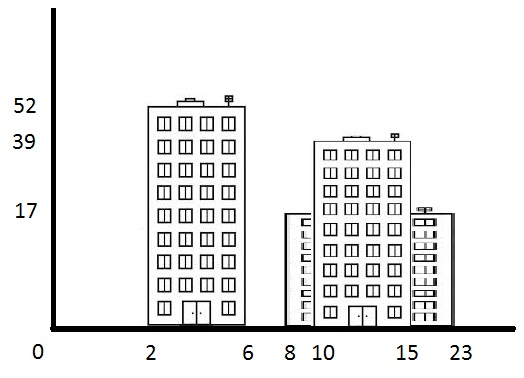
\includegraphics[scale=0.7]{./Imagenes/Ej1/ediRandom}
  \caption{}
  \label{fig:ejemplo}
\end{figure}  
    
  
  
  \item \textbf{Edificios} espaciados de a pares (es decir $\forall e1, e2 \in Edificios, e1 \neq e2, der(e1) < izq(e2) \bigwedge izq(e1) < izq(e2) \bigwedge der(e1) < der(e2)$ )
    
\begin{figure}[H]
  \centering
    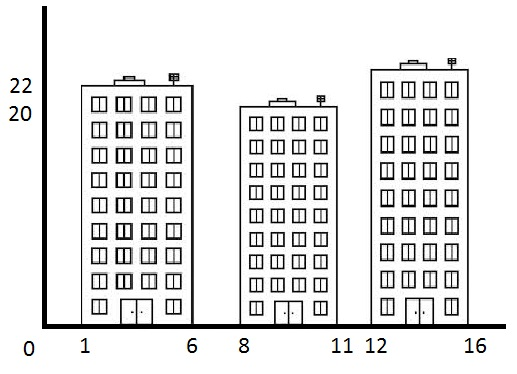
\includegraphics[scale=0.7]{./Imagenes/Ej1/ediSeparado}
  \caption{}
  \label{fig:ejemplo}
\end{figure}
  
  \item \textbf{Edificios} formando una escalera descendente, (es decir $\forall e1, e2 \in Edificios, e1 \neq e2, izq(e1) < izq(e2) \bigwedge der(e1) < der(e2) \bigwedge alt(e1) < alt(e2) $)
	
	\begin{figure}[H]
  \centering
    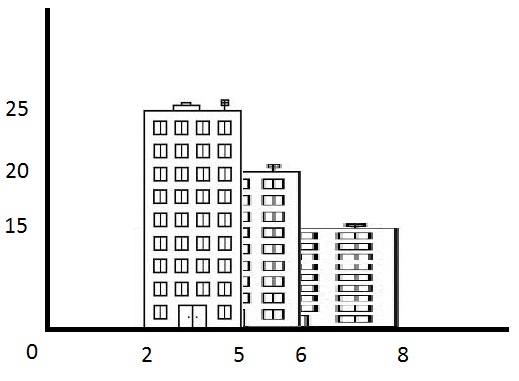
\includegraphics[scale=0.7]{./Imagenes/Ej1/ediEscalera}
  \caption{}
  \label{fig:ejemplo}
\end{figure}  
  
\end{enumerate}

Para verificar que nuestra complejidad teórica se verifica en la práctica, lo que tratamos fue de "`linealizar"' las muestras. Es decir, si la muestra $m_{i}$ es $O(n logn)$ entonces graficando $\frac{m_{i}}{(n logn)}$ deberíamos obtener una recta (esto se puede visualizar en la figura GG). 

\begin{figure}[H]
	\centering
	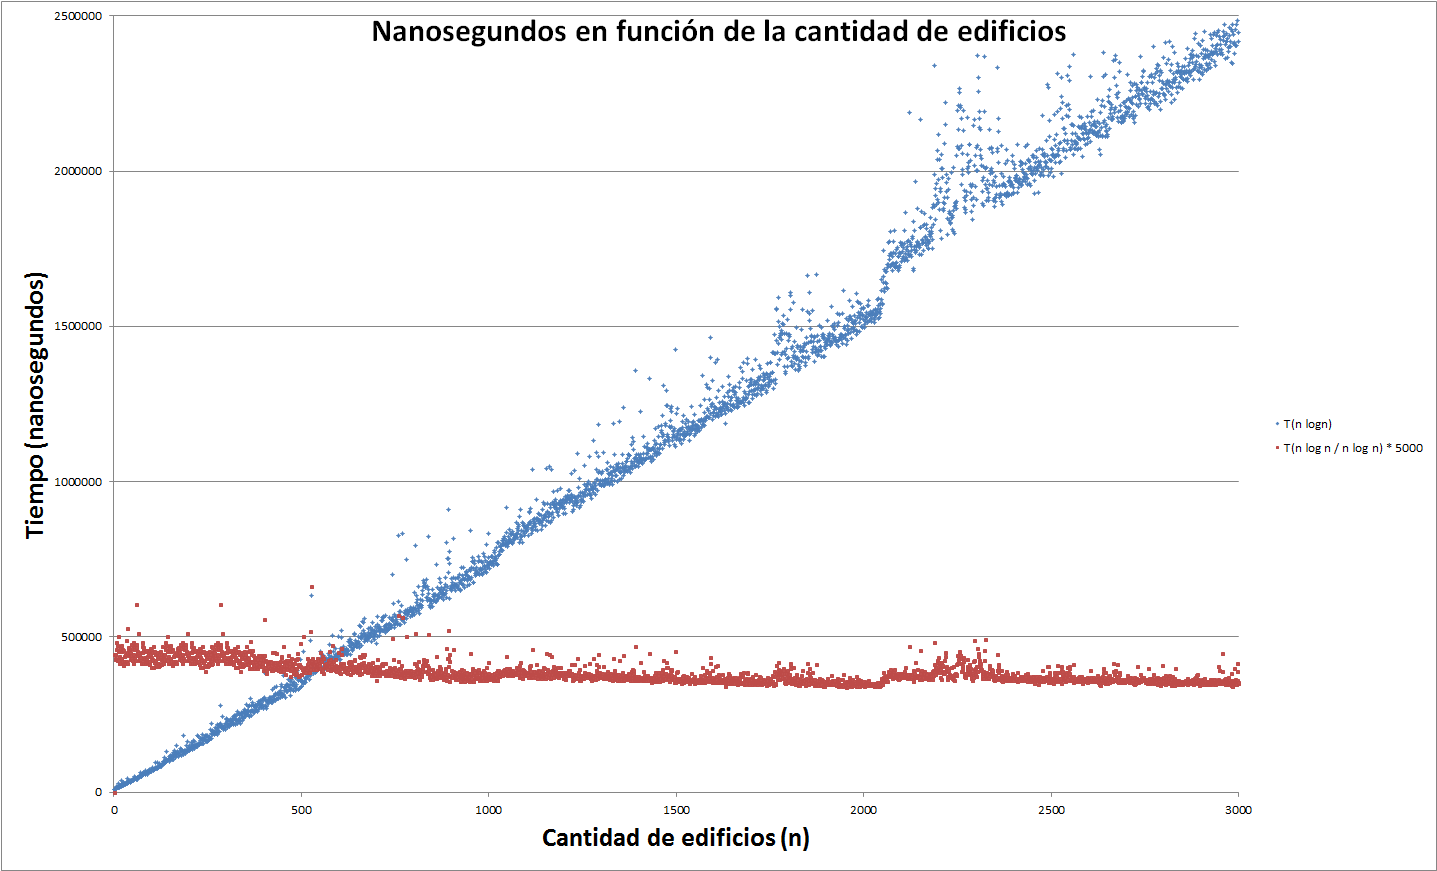
\includegraphics[scale=0.45]{Imagenes/Ej2/exp2_random.png}
	\caption{Comparación de tiempos}
	\label{fig:ej1_comple2}
\end{figure}
Notar que al graficar $T(n logn)/n logn$ se la multiplica por 5000 para que el gráfico pueda ser apreciado con fácilidad.
Ahora bien, nos resulto interesante realizar experimentos para distintos tipos de entrada. Dados los conjuntos de entradas antes descriptos, mostramos los resultados que obtuvimos:

\begin{figure}[H]
	\centering
	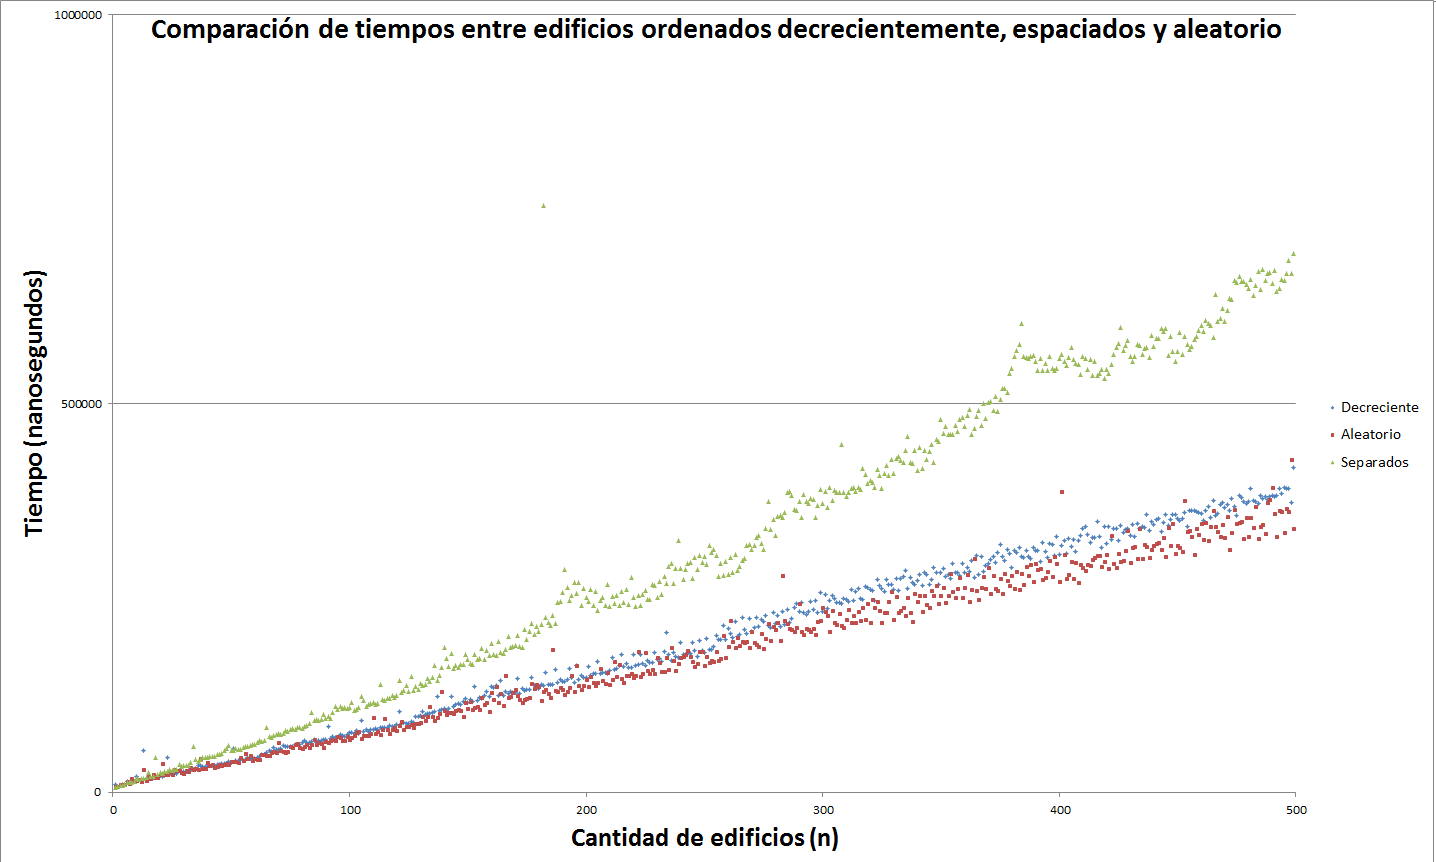
\includegraphics[scale=0.45]{Imagenes/Ej2/exp2_comparacion.png}
	\caption{Comparación de tiempos}
	\label{fig:ej1_comple2}
\end{figure}

\begin{figure}[H]
	\centering
	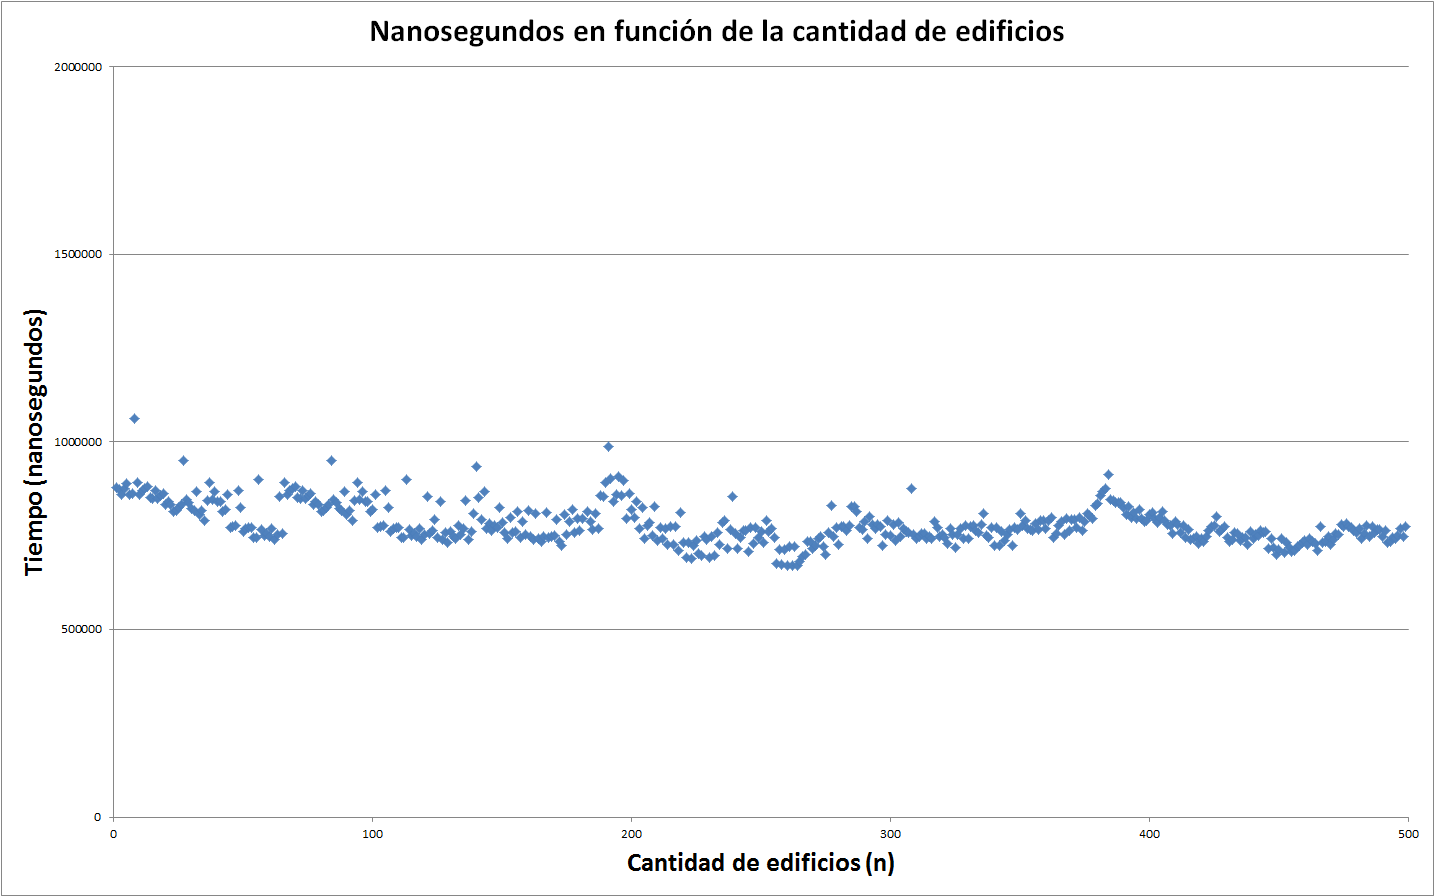
\includegraphics[scale=0.45]{Imagenes/Ej2/exp2_sep_const.png}
	\caption{Comparación de tiempos}
	\label{fig:ej1_comple2}
\end{figure}
